\section{Results}
\label{sec:results}
\paragraph{Performance metrics}
 \Cref{fig:retrieval} shows performance of the basic model on
 retrieval; \Cref{fig:triplet} shows the scores for the triplet
 task. It can be seen that for both types of validation datasets
 (dialog and narration) the triplet scores are substantially above
 chance. In the case of the narration data this scores is not
 confounded by speaker-based clues, which is a indication that the
 model possibly learned to detect some aspects of utterance
 meaning. We investigate this hypothesis further using multiple
 representational similarity analysis.
 

\begin{figure}
  \centering
  \begin{tabular}{cc}
    Dialog & Narration \\
    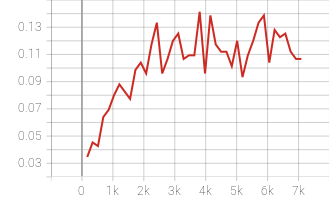
\includegraphics[scale=0.3]{val_rec10.png} & 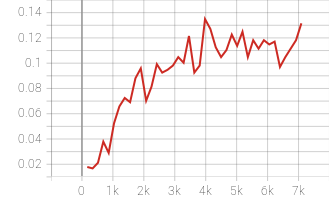
\includegraphics[scale=0.3]{valnarr_rec10.png}\\
  \end{tabular}
  \caption{Validation recall@10 on the retrieval task. The x-axis
    shows the training steps.}
  \label{fig:retrieval}
\end{figure}

\begin{figure}
  \centering
  \begin{tabular}{cc}
    Dialog & Narration \\
    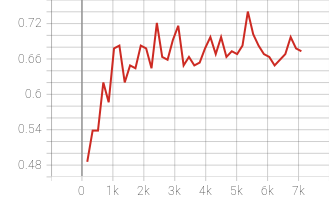
\includegraphics[scale=0.3]{val_acc3.png}  & 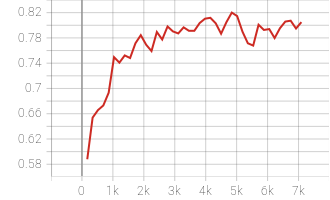
\includegraphics[scale=0.3]{valnarr_acc3.png}\\
  \end{tabular}
  \caption{Validation accuracy on the triplet task. The x-axis shows
    the training steps.}
  \label{fig:triplet}
\end{figure}

\paragraph{Multiple representational similarity analysis}
\Cref{tab:dialog-lm} and \Cref{tab:narration-lm} show the coefficients
of the linear models fit to the dialog and narration pairwise
similarity data respectively. For both datasets the predictors with
the largest effects in terms of standardized coefficient magnitude and
partial $R^2$ are {\tt durationdiff} and {\tt glovesim}
(\Cref{fig:sim-glove-duration} plots the pairwise similarities
against these two variable to illustrate the details of the
relationship).
 
The effect of
the {\tt samespeaker} predictor for the dialog data is negative and
small in size.  These results further indicate that the model learns
some aspects of word-level semantics as captured by GloVe word
vectors, and that speaker identity does not appear to be a substantial
impact on utterance embeddings.

Perhaps unexpectedly, the predictor meant to capture phonemic distance
{\tt distance} is not strongly associated with utterance similarity,
although it should be noted that here we are only investigating model
embeddings after the final attention pooling layer.The strength of
the association between differences in utterance duration {\tt
  durationdiff} and pairwise similarities apparent in this data was
suprising and possibly undesirable, and thus warrants further investigation.



\begin{table}
  \centering
\begin{tabular}{lrrrrr}
\toprule
  & Estimate & Std. Error & t value & Pr(>|t|) & partial\_r2\\
\midrule
(Intercept) & 0.008 & 0.009 & 0.814 & 0.415 & 0.000\\
glovesim & 0.064 & 0.001 & 52.404 & 0.000 & 0.006\\
distance & 0.002 & 0.001 & 1.718 & 0.086 & 0.000\\
durationdiff & -0.589 & 0.001 & -491.729 & 0.000 & 0.348\\
sametype & -0.001 & 0.009 & -0.084 & 0.933 & 0.000\\
\addlinespace
samespeaker & -0.013 & 0.002 & -7.164 & 0.000 & 0.000\\
sameepisode & 0.029 & 0.002 & 18.568 & 0.000 & 0.001\\
\bottomrule
\end{tabular}
\caption{Association of predictors with model-based pairwise
  similarity scores for single-word utterances in the dialog
  validation data. Indicators are sum-coded ($1$ vs $-1$) while the
  numerical variables are z-scored.}
\label{tab:dialog-lm}
\end{table}

%> rawdata.d <- read.csv("pairwise_similarities_dialog.csv")
%> data <- rawdata.d %>% filter(durationdiff<0.001 & glovesim != 0)
%> cor(data$similarity, data$glovesim)
%[1] 0.109515


\begin{table}
  \centering

\begin{tabular}{lrrrrr}
\toprule
  & Estimate & Std. Error & t value & Pr(>|t|) & partial\_r2\\
\midrule
(Intercept) & -0.082 & 0.001 & -65.693 & 0 & 0.000\\
glovesim & 0.186 & 0.000 & 1027.442 & 0 & 0.037\\
distance & 0.008 & 0.000 & 38.478 & 0 & 0.000\\
durationdiff & -0.467 & 0.000 & -2806.787 & 0 & 0.224\\
sametype & -0.157 & 0.001 & -154.327 & 0 & 0.001\\
\addlinespace
sameepisode & 0.073 & 0.001 & 95.065 & 0 & 0.000\\
\bottomrule
\end{tabular}
\caption{Association of predictors with model-based pairwise
  similarity scores for single-word utterances in the narration
  validation data. Indicators are sum-coded ($1$ vs $-1$) while the
  numerical variables are z-scored.}
\label{tab:narration-lm}
\end{table}

%       Correlation for duration-matched pairs:
% > data <- rawdata.n %>% filter(durationdiff<0.001 & glovesim != 0)
% > cor(data$similarity, data$glovesim)
% 0.3665952

\begin{figure}
  \centering
  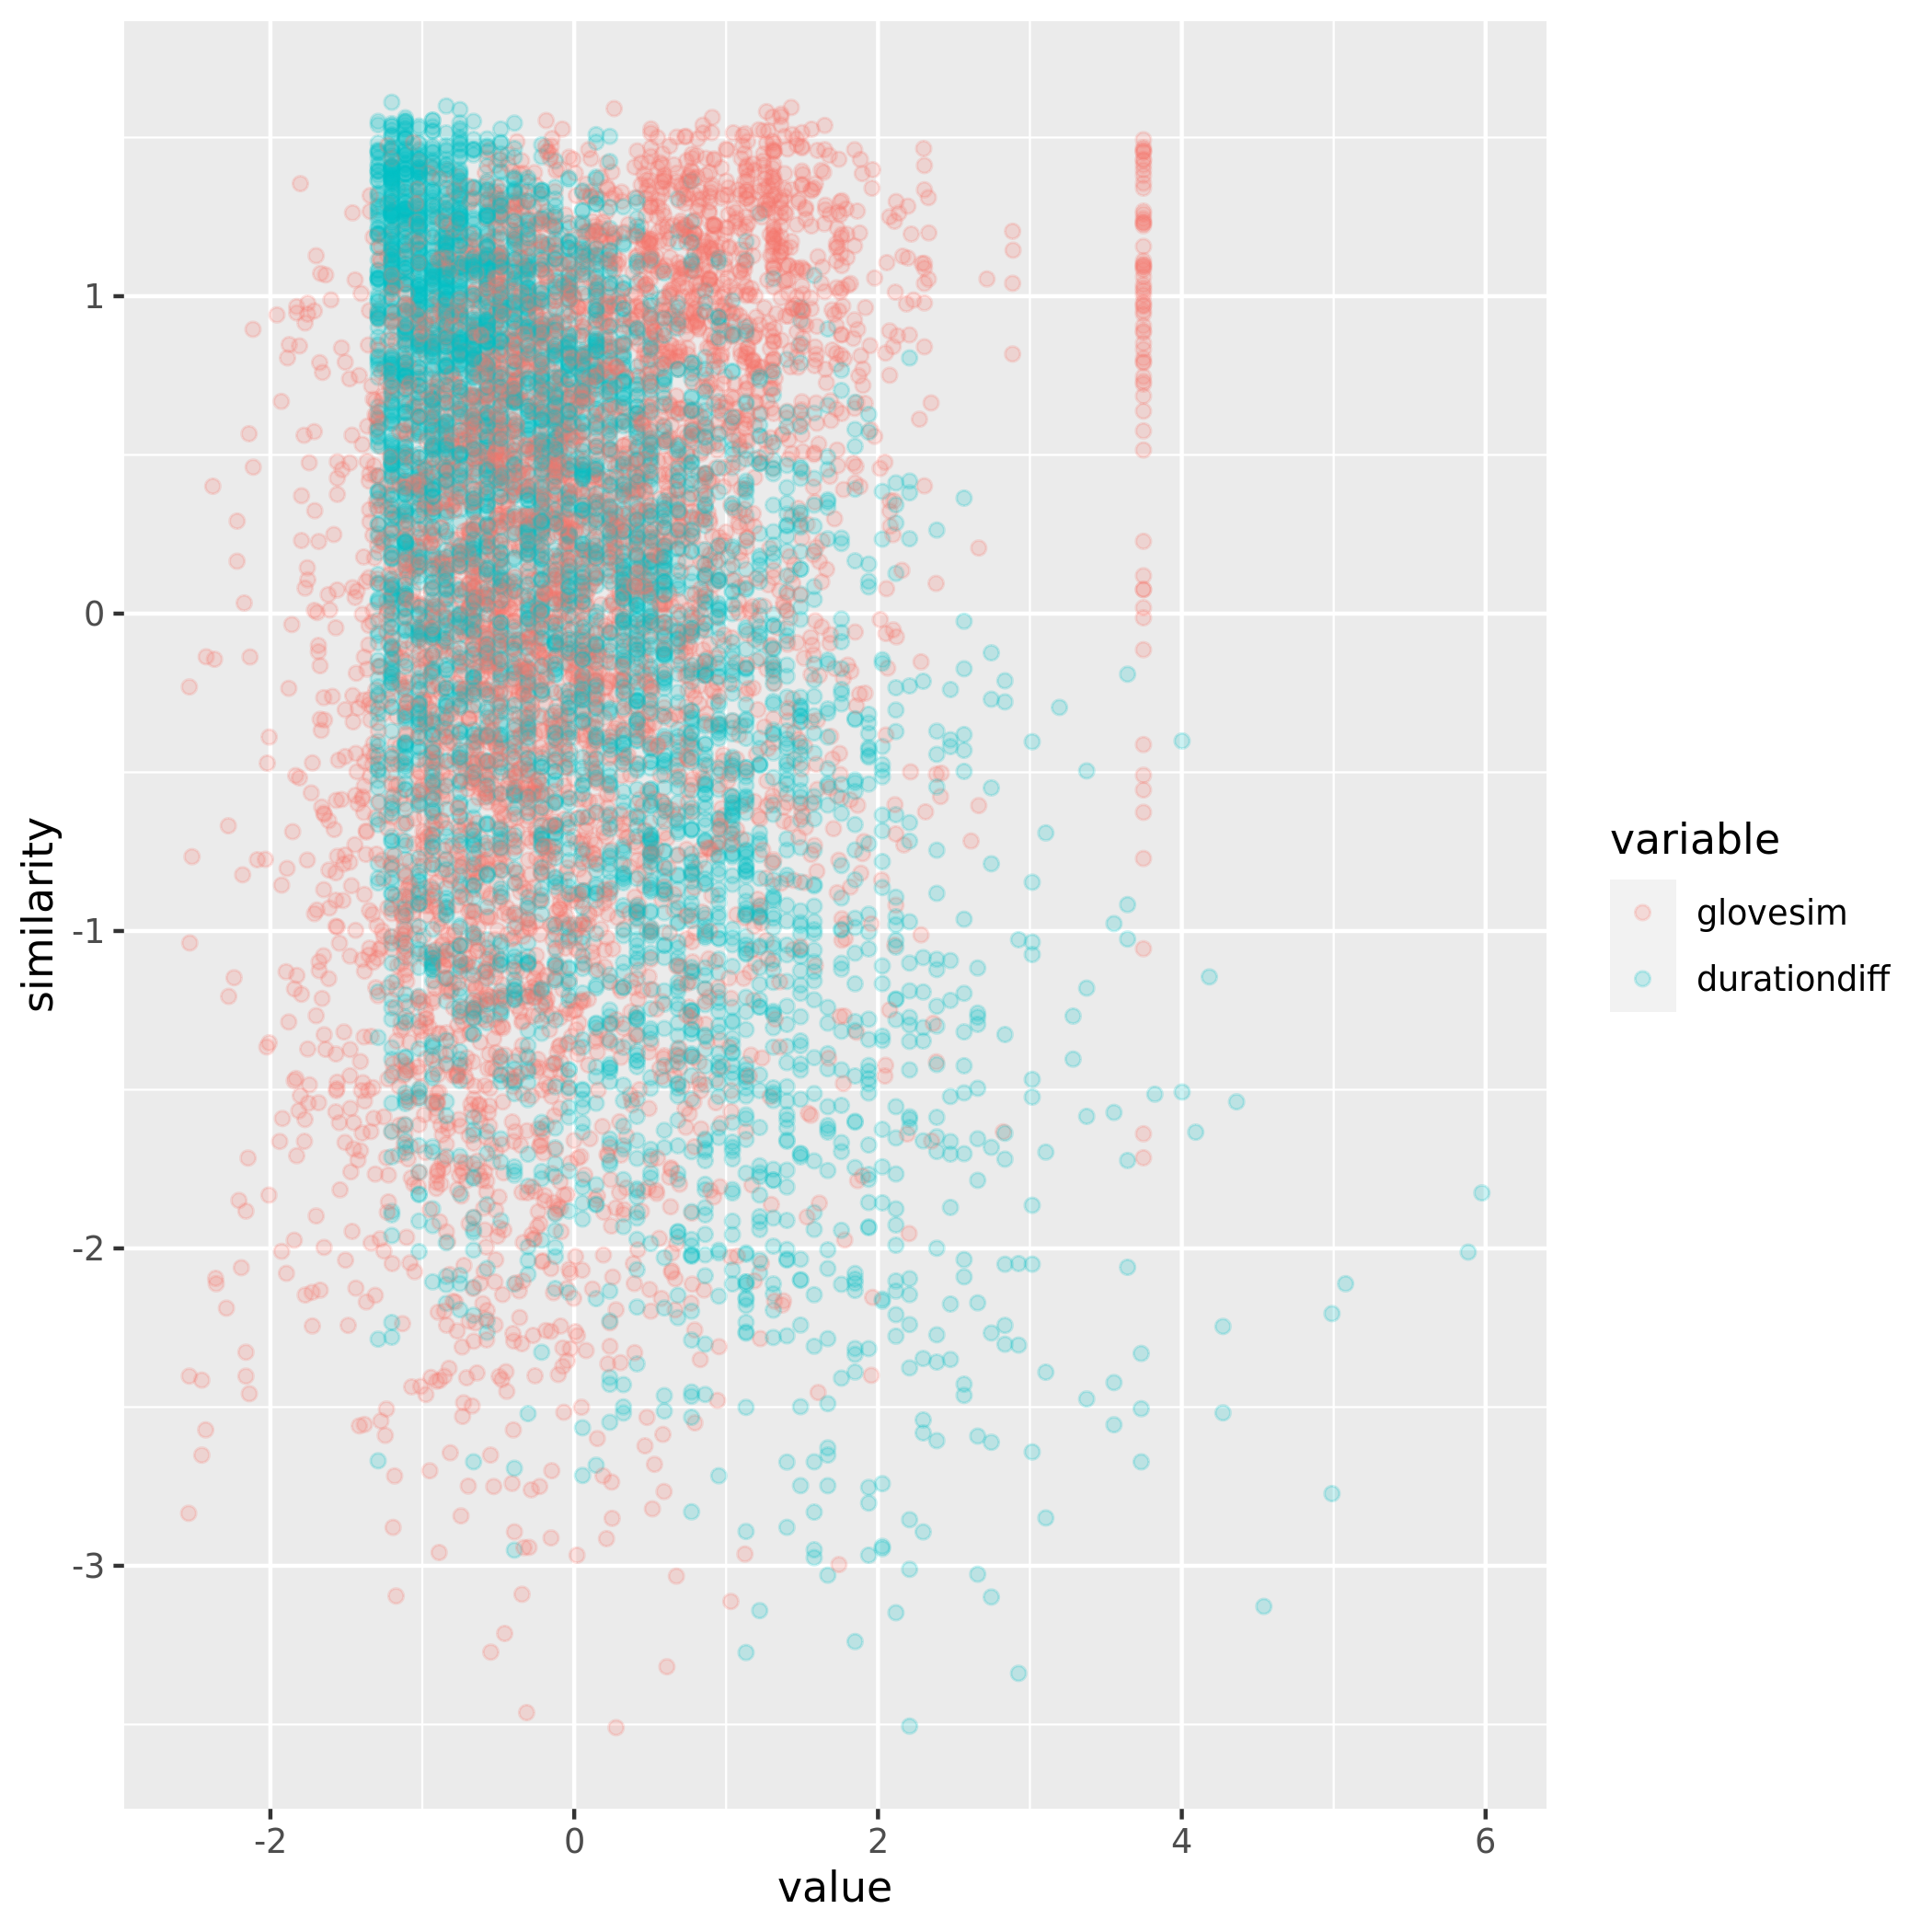
\includegraphics[scale=0.6]{sim-glove-duration.png}
  \caption{The relationship between pairwise {\tt similarity} and the
    two variables with the strongest association with it, {\tt
      glovesime} and {\tt durationdiff} (narration data). All
    variables z-scored.}
  \label{fig:sim-glove-duration}
\end{figure}